% =====================================================================
%  How the mem-X memory wrapper CONNECTS to the frozen base (simple view)
%  Kept in sync with wrapper-connect.png (used in slides/weekly/v1.5-gating.tex).
%  Compile standalone (Overleaf / pdflatex) to regenerate the figure.
% =====================================================================
\documentclass[tikz,border=8pt]{standalone}
\usetikzlibrary{arrows.meta, positioning}
\begin{document}
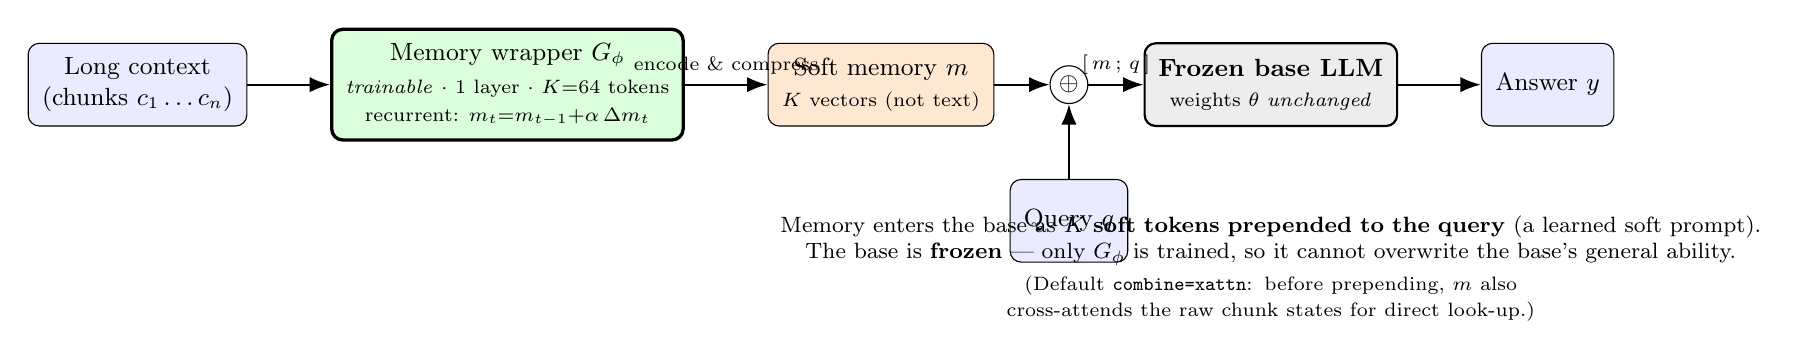
\begin{tikzpicture}[
  font=\small,
  box/.style   ={draw, rounded corners, align=center, minimum height=1.05cm, inner sep=5pt},
  ctx/.style   ={box, fill=blue!8},
  train/.style ={box, fill=green!14, very thick},
  mem/.style   ={box, fill=orange!18},
  frozen/.style={box, fill=gray!14, thick},
  arr/.style   ={-{Latex[length=2.6mm]}, thick},
  node distance=0.85cm and 1.05cm,
]
  \node[ctx]                       (chunks){Long context\\(chunks $c_1\dots c_n$)};
  \node[train, right=of chunks]    (wrap)  {Memory wrapper $G_\phi$\\[1pt]\scriptsize\emph{trainable} $\cdot$ 1 layer $\cdot$ $K{=}64$ tokens\\[-1pt]\scriptsize recurrent: $m_t{=}m_{t-1}{+}\alpha\,\Delta m_t$};
  \node[mem, right=of wrap]        (mem)   {Soft memory $m$\\\scriptsize $K$ vectors (not text)};
  \node[draw, circle, inner sep=1.5pt, right=0.7cm of mem] (cc){$\oplus$};
  \node[frozen, right=0.7cm of cc] (base)  {\textbf{Frozen base LLM}\\\scriptsize weights $\theta$ \emph{unchanged}};
  \node[ctx, right=of base]        (ans)   {Answer $y$};
  \node[ctx, below=0.95cm of cc]   (q)     {Query $q$};

  \draw[arr] (chunks) -- (wrap);
  \draw[arr] (wrap)   -- node[above]{\scriptsize encode \& compress} (mem);
  \draw[arr] (mem)    -- (cc);
  \draw[arr] (q)      -- (cc);
  \draw[arr] (cc)     -- node[above]{\scriptsize $[\,m\,;\,q\,]$} (base);
  \draw[arr] (base)   -- (ans);

  \node[align=center, below=1.0cm of base, text width=12.5cm, font=\footnotesize]
    {Memory enters the base as $K$ \textbf{soft tokens prepended to the query} (a learned soft prompt).
     The base is \textbf{frozen} --- only $G_\phi$ is trained, so it cannot overwrite the base's general ability.\\[2pt]
     {\scriptsize (Default \texttt{combine=xattn}: before prepending, $m$ also cross-attends the raw chunk states for direct look-up.)}};
\end{tikzpicture}
\end{document}
